%!TEX program = xelatex
\documentclass[dvipsnames, svgnames,a4paper,11pt]{article}
% ----------------------------------------------------
%   中山大学物理与天文学院本科实验报告模板
%   作者:Huanyu Shi,2019级
%   知乎:https://www.zhihu.com/people/za-ran-zhu-fu-liu-xing
%   Github:https://github.com/Huanyu-Shi/SYSU-SPA-Labreport-Template
%   Last update : 2023.4.10
% ----------------------------------------------------

% ----------------------------------------------------- 
%	加边框的命令
%	参考:https://tex.stackexchange.com/questions/531559/how-to-add-the-page-border-for-first-two-pages-in-latex
\usepackage{tikz}
\usetikzlibrary{calc}
\usepackage{eso-pic}
\AddToShipoutPictureBG{%
\begin{tikzpicture}[overlay,remember picture]
\draw[line width=0.6pt] % 边框粗细
    ($ (current page.north west) + (0.6cm,-0.6cm) $)
    rectangle
    ($ (current page.south east) + (-0.6cm,0.6cm) $); % 边框位置
\end{tikzpicture}}


\usepackage{xcolor}
\definecolor{c1}{HTML}{2752C9} % 目录颜色
\definecolor{c2}{RGB}{190,20,83} % 引用颜色

\usepackage{ctex}
\usepackage[top=28mm,bottom=28mm,left=15mm,right=15mm]{geometry}
\usepackage{hyperref} 
\hypersetup{
	colorlinks,
	linktoc = section, % 超链接位置,选项有section, page, all
	linkcolor = c1, % linkcolor 目录颜色
	citecolor = c1  % citecolor 引用颜色
}
\usepackage{amsmath,enumerate,multirow,float}
\usepackage{tabularx}
\usepackage{tabu}
\usepackage{subfig}
\usepackage{fancyhdr}
\usepackage{graphicx}
\usepackage{wrapfig}  
\usepackage{physics}
\usepackage{appendix}
\usepackage{amsfonts}

%
\usepackage{tcolorbox}
\tcbuselibrary{skins,breakable}
\newtcolorbox{tbox}[2][]{
    colframe=black!70!,
    breakable,
    enhanced,
	boxrule =0.5pt,
    title = {#2},
    fonttitle = \large\kaishu\bfseries,
	drop fuzzy shadow,
    #1
}
\newtcolorbox[auto counter,number within=section]{question}[1][]{
  top=2pt,bottom=2pt,arc=1mm,
  boxrule=0.5pt,
%   frame hidden,
  breakable,
  enhanced, %跨页后不会显示下边框
  coltitle=c1!80!gray,
  colframe=c1,
  colback=c1!3!white,
  drop fuzzy shadow,
  title={思考题~\thetcbcounter:\quad},
  fonttitle=\bfseries,
  attach title to upper,
  #1
}
\newcommand{\setLhead}[1]{%
  \lhead{{\color{gray}\kaishu #1}} % 定义新的命令,设置右边页眉的内容
}
\newcommand{\setRhead}[1]{%
  \rhead{{\color{gray}\kaishu #1}} % 定义新的命令,设置右边页眉的内容
}
% ---------------------------------------------------------------------
%	利用cleveref改变引用格式,\cref是引用命令
\usepackage{cleveref}
\crefformat{figure}{#2{\textcolor{c2}{图 #1}}#3} % 图片的引用格式
\crefformat{equation}{#2{(\textcolor{c2}{#1})}#3} % 公式的引用格式
\crefformat{table}{#2{\textcolor{c2}{表 #1}}#3} % 表格的引用格式


% ---------------------------------------------------------------------
%	页眉页脚设置
\fancypagestyle{plain}{\pagestyle{fancy}}
\pagestyle{fancy}
\setLhead{中山大学物理与天文学院基础物理实验预习报告}
%\lhead{\kaishu 中山大学物理与天文学院物理实验\uppercase\expandafter{\romannumeral3}} % 左边页眉,学院 + 课程
%\rhead{{\color{gray}\kaishu Template 实验报告模板}} % 右边页眉,实验报告标题
\setRhead{实验1\hspace{1pt}冰的熔化热测量}
\cfoot{\thepage} % 页脚,中间添加页码


% ---------------------------------------------------------------------
%	对目录、章节标题的设置
\renewcommand{\contentsname}{\centerline{\huge 目录}}
\usepackage{titlesec}
\usepackage{titletoc}
% \titleformat{章节}[形状]{格式}{标题序号}{序号与标题间距}{标题前命令}[标题后命令]
\titleformat{\section}{\centering\LARGE\songti}{}{1em}{}

% ---------------------------------------------------------------------
%   listing代码环境设置
\usepackage{listings}
\lstloadlanguages{python}
\lstdefinestyle{pythonstyle}{
backgroundcolor=\color{gray!5},
language=python,
frameround=tftt,
frame=shadowbox, 
keepspaces=true,
breaklines,
columns=spaceflexible,                   
basicstyle=\ttfamily\small, % 基本文本设置,字体为teletype,大小为scriptsize
keywordstyle=[1]\color{c1}\bfseries, 
keywordstyle=[2]\color{Red!70!black},   
stringstyle=\color{Purple},       
showstringspaces=false,
commentstyle=\ttfamily\scriptsize\color{green!40!black},%注释文本设置,字体为sf,大小为smaller
tabsize=2,
morekeywords={as},
morekeywords=[2]{np, plt, sp},
numbers=left, % 代码行数
numberstyle=\it\tiny\color{gray}, % 代码行数的数字字体设置
stepnumber=1,
rulesepcolor=\color{gray!30!white}
}




% ---------------------------------------------------------------------
%	其他设置
\def\degree{${}^{\circ}$} % 角度
\graphicspath{{./images/}} % 插入图片的相对路径
\allowdisplaybreaks[4]  %允许公式跨页 % 导入模板的相关设置
\usepackage{lipsum}
\usepackage{indentfirst}
\usepackage{pdfpages}
\usepackage{multirow}
\usepackage{subfig}
\usepackage{graphicx}
\usepackage{float} 
\usepackage{booktabs}
\usepackage{enumerate}
\usepackage{makecell} 
\renewcommand{\d}{\mathrm{d}}
\newcommand{\upcite}[1]{\textsuperscript{\textsuperscript{\cite{#1}}}}


%---------------------------------------------------------------------
%	正文
%---------------------------------------------------------------------
\newcommand{\exname}{基尔霍夫定律和叠加原理}%实验名称
\setRhead{\exname}
\begin{document}


\begin{table}
	\renewcommand\arraystretch{1.7}
	\begin{tabularx}{\textwidth}{
		|X|X|X|X
		|X|X|X|X|}
	\hline
	\multicolumn{2}{|c|}{预习报告}&\multicolumn{2}{|c|}{实验记录}&\multicolumn{2}{|c|}{分析讨论}&\multicolumn{2}{|c|}{总成绩}\\
	\hline
	 \hspace{0.625cm}25& & \hspace{0.625cm}35  & & \hspace{0.625cm}30  & &  \hspace{0.625cm}90 & \\
	\hline
	\end{tabularx}
\end{table}


\begin{table}
	\renewcommand\arraystretch{1.7}
	\begin{tabularx}{\textwidth}{|X|X|X|X|}
	\hline
	年级、专业:& 2023级物理学类 &组号:& \\
	\hline
	姓名:& 姚昊廷、李风磊 & 学号:&22322091、23344083\\
	\hline
	日期:&2025.3.12  & 教师签名:& \\
	\hline
	\end{tabularx}
\end{table}

\begin{center}
	\LARGE \exname
\end{center}

\textbf{【实验报告注意事项】}
\begin{enumerate}
	\item 实验报告由三部分组成:
	\begin{enumerate}
		\item 预习报告:课前认真研读\underline{\textbf{实验讲义}},弄清实验原理;实验所需的仪器设备、用具及其使用、完成课前预习思考题;了解实验需要测量的物理量,并根据要求提前准备实验记录表格。
	    \item 实验记录:认真、客观记录实验条件、实验过程中的现象以及数据。实验记录请用珠笔或者钢笔书写并签名(\textcolor{red}{\textbf{用铅笔记录的被认为无效}})。\textcolor{red}{\textbf{保持原始记录,包括写错删除部分,如因误记需要修改记录,必须按规范修改。}}(不得手记的值输入到电脑打印);离开前请实验教师检查记录并签名。
	    \item 数据处理及分析讨论:处理实验原始数据(学习仪器使用类型的实验除外),对数据的可靠性和合理性进行分析;按规范呈现数据和结果(图、表),包括数据、图表按顺序编号及其引用;分析物理现象(含回答实验思考题,写出问题思考过程,必要时按规范引用数据);最后得出结论。
	\end{enumerate}
	\textbf{实验报告就是将预习报告、实验记录、和数据处理与分析合起来,加上本页封面。}
	\item 实验报告在\textcolor{red}{\textbf{每个小结(补做)的之后一周内}}提交,最后一次实验,在\textcolor{red}{\textbf{结束一周内}}提交。
	\item 注意事项:\begin{enumerate}
		\item 请认真查看并理解\textcolor{red}{\textbf{实验讲义第一章}}内容
		\item 注意实验器材的合理使用。
		\item 使用结束使用各种仪器之后需要将其放回原位
	\end{enumerate}
\end{enumerate}



\clearpage
\tableofcontents
\clearpage

\setcounter{section}{0}
\section{\exname\ \textbf{预习报告}}
	
\subsection{实验目的}
\begin{enumerate}
    \item 加深对基尔霍夫定律的理解。
    \item 学习验证定律的方法和仪器仪表的正确使用。
    \item 研究叠加原理的成立条件并在线性电路中验证叠加原理。
\end{enumerate}
\subsection{仪器用具}
\begin{table}[htbp]
	\centering
	\renewcommand\arraystretch{1.6}
	% \setlength{\tabcolsep}{10mm}
	\begin{tabular}{p{0.05\textwidth}|p{0.20\textwidth}|p{0.05\textwidth}|p{0.5\textwidth}}
	\hline
	编号& 仪器用具名称 & 数量 &  主要参数(型号,测量范围,测量精度等) \\
	\hline
	1&电路原理箱或板&1 &\\
	\hline
    2&稳压源&1 &\\
	\hline
    3&直流电流源&1 &\\
	\hline
    4&直流电流表&1 &\\
	\hline
    5&直流电压表&1 &\\
	\hline
    6&电流表专用线&1 &\\
	\hline
    7&2号实验导线&1 &\\
	\hline
    8&其他&1 &\\
	\hline
\end{tabular}
\end{table}


\subsection{原理概述}
\begin{enumerate}
    \item 基尔霍夫定律是集总电路的基本定律,包括电流定律(KCL)和电压定律(KVL)。\par
    基尔霍夫定律规定了电路中各支路电流之间和各支路电压之间必须服从的约束关系,无论电路元件是线性的或是非线性的,时变的或是非时变的,只要电路是集总参数电路,都必须服从这个约束关系。
    \begin{enumerate}
        \item 基尔霍夫电流定律(KCL)。在集总电路中,任何时刻,对任一节点,所有支路电流的代数和恒等于零,即$\sum i=0$。通常约定,流出节点的支路电流取正号,流入节点的支路电流取负号。
        \item 基尔霍夫电压定律(KVL)。在集总电路中,任何时刻,沿任一回路所有支路电压的代数和恒等于零,即沿任一回路有$\sum u=0$。在写此式时,首先需要任意指定一个回路绕行的方向。凡电压的参考方向与回路绕行方向一致者,取“+”号;电压参考方向与回路绕行方向相反者,取“-”号。
        \item KCL和KVL定律适用于任何集总参数电路,而与电路中的元件的性质和参数大小无关,不管这些元件是线性的、非线性的、含源的、无源的、时变的、非时变的等,定律均适用。
    \end{enumerate}
    \item 叠加原理\par
    对于一个线性系统,一个含多个独立源的线性电路的任何支路的响应(电压或电流),等于每个独立源单独作用时的响应的代数和,此时所有其他独立源被替换成他们各自的阻抗。\par
    叠加原理成立的条件是:线性系统;线性系统具有比例性和可加性,由线性元件组成的电路系统是线性系统,如由电源和普通电阻组成的系统在温度恒定的环境中可以认定为是线性系统;如果电路中有非线性元件,如二极管,则电路不是线性系统。

\end{enumerate}
\subsection{实验预习题}
\begin{question}
    画出实验电路图,标明选用的电路参数、电流方向、回路绕行方向和所选节点与回路名称等。
    \tcblower
    \begin{figure}[H]
        \centering
        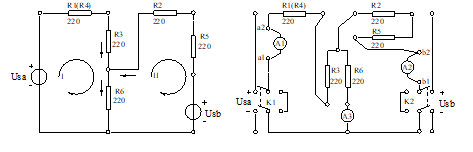
\includegraphics[width=0.8\textwidth]{实验2图片1.png}
        \caption{实验电路图}
    \end{figure}
\end{question}

\begin{question}
    用PROTEUS开展仿真实验。
    \tcblower
    \begin{figure}[H]
        \centering
        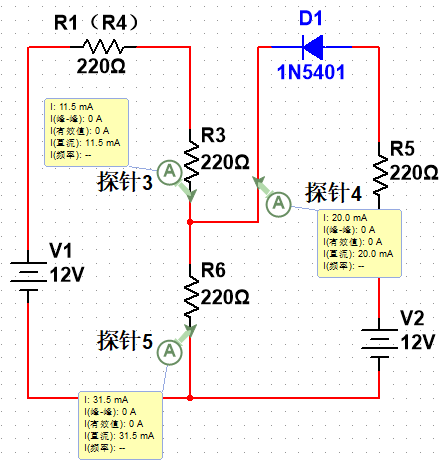
\includegraphics[width=0.4\textwidth]{实验2图片2.png}
        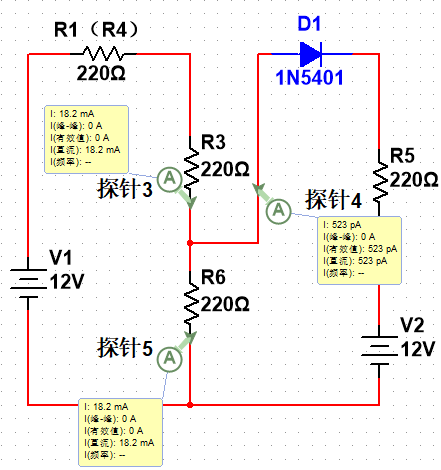
\includegraphics[width=0.4\textwidth]{实验2图片3.png}
        
    \end{figure}
    \begin{figure}[H]
        \centering
        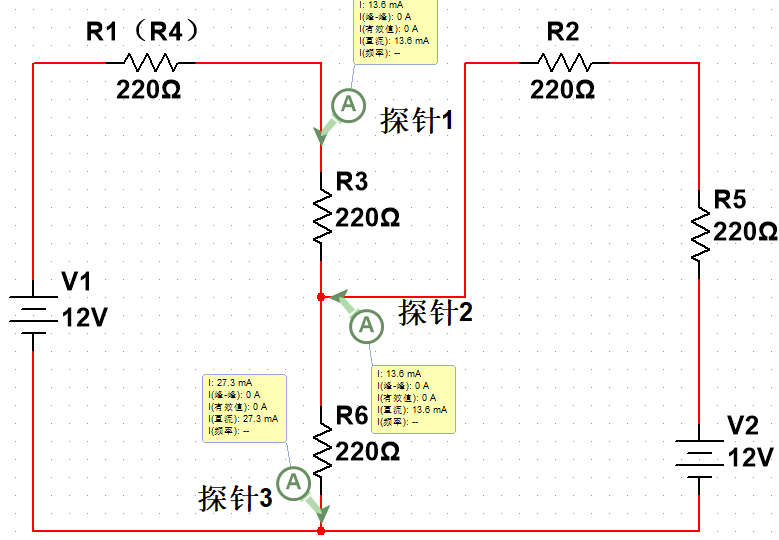
\includegraphics[width=0.4\textwidth]{实验2图片4.png}
        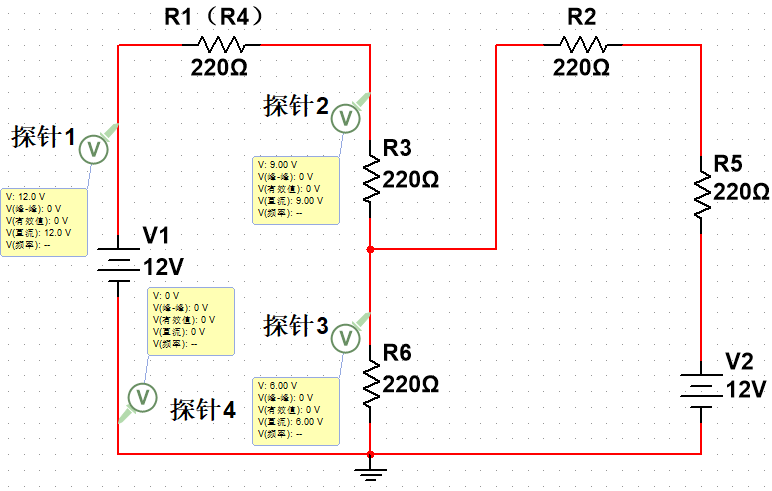
\includegraphics[width=0.4\textwidth]{实验2图片5.png}
        \caption{仿真计算图}
    \end{figure}
\end{question}
\begin{question}
    对实验电路进行理论计算,并比较计算值与仿真结果。
    \tcblower
    由线性叠加原理知经过$R_3$的电流为$\frac{3U_{sa}}{1760}-\frac{U_{sb}}{1760}$,经过$R_2$的电流为$\frac{3U_{sb}}{1760}-\frac{U_{sa}}{1760}$,经过$R_6$的电流为$\frac{U_{sa}+U_{sb}}{880}$。
    代入$U_{sa}=12\text{V},U_{sb}=12\text{V}$可得
    \begin{align*}
        i_1&=13.6\text{mA}\\
        i_2&=13.6\text{mA}\\
        i_3&=27.3\text{mA}
    \end{align*}
    与仿真结果相同
\end{question}


\begin{question}
    根据理论计算和仿真结果,确定实验过程中各个步骤的电源参数和电阻参数。
    \tcblower
    在确保不超过万用表量程的情况下,应尽可能选择较为大的电源电压和较小的电阻。
\end{question}
\clearpage
\setLhead{中山大学物理与天文学院基础物理实验记录}
\begin{table}
	\renewcommand\arraystretch{1.7}
	\centering
	\begin{tabularx}{\textwidth}{|X|X|X|X|}
	\hline
	专业:& 物理学类 &年级:& 2023级 \\
	\hline
	姓名:& 姚昊廷、李风磊 & 学号:&22322091、23344083\\
	\hline
	室温:&$22^\circ$C&实验地点:&\\
	\hline
	学生签名:& & 评分: &\\
	\hline
	实验时间:&2025.3.12  & 教师签名:&\\
	\hline
	\end{tabularx}
\end{table}
\section{\exname\ \textbf{实验记录}}
\subsection{实验内容、步骤、结果}
实验步骤:
\begin{enumerate}
	\item 线性电路的KCL,KVL和叠加原理\\
	设计电路图如下
	\vspace{10cm}
	并按电路图连线
	\begin{enumerate}
		\item 验证(KCL)定律,即$\sum i=0$。在电路中,选择R2,R3,R6公共连接点作为测试点,测量流入流出该节点的各支路电流数值和方向(注意电流表的表笔对应的正负),记录数据并进行验证。
		\item 验证(KVL)定律,即$\sum u=0$。在电路中任选一网孔(回路),测量网孔内所有支路的元件电压值和电压方向,对应记入附表并进行验证。
		\item 验证叠加定理。参考电路中,电路中电源$U_{sa}$、$U_{sb}$是由实验室数控直流稳压电源供电,在正常恒压输出模式时上一次实验已经验证为理想电压源;其他元件都是电阻,在实验室条件下,可以认为是线性元件。所以,参考实验电路可以认定为线性系统。
		\item 不改变电路结构,只改变电源$U_{sa}$、$U_{sb}$的值和电阻的阻值
	\end{enumerate}
	\item 非线性电路的KCL,KVL和叠加原理
	\begin{enumerate}
		\item 把实验电路中的电阻R2替换为二极管(1N5401,在元件伏安特性模块),重复进行上述实验((a)(b)(c))。
		\item 把代替了电阻R2的二极管(1N5401)反向接入电路,再重复进行上述实验((a)(b)(c))。
	\end{enumerate}
\end{enumerate}
\newpage
\vspace*{\fill}
\subsection{实验过程遇到问题及解决办法}
\vspace*{\fill}
\clearpage
\setLhead{中山大学物理与天文学院基础物理实验分析与讨论}
\begin{table}
	\renewcommand\arraystretch{1.7}
	\begin{tabularx}{\textwidth}{|X|X|X|X|}
	\hline
	专业:& 物理学 &年级:& 2023级\\
	\hline
	姓名:& 姚昊廷、李风磊 & 学号:&22322091、23344083\\
	\hline
    日期:&2025.3.12 &  &\\
	\hline
	评分:&&教师签名:&\\
	\hline
	\end{tabularx}
\end{table}

\section{\exname\ \textbf{分析与讨论}}
\subsection{分析与讨论}
\newpage
\vspace*{\fill}
\subsection{实验心得和体会、意见建议等}
\vspace*{\fill}
\clearpage
% ---------------------------------------------------------------------
%   参考文献
%   注:使用参考文献时应按照xelatex->bibtex->xelatex->xelatex顺序进行编译
%\phantomsection
%\addcontentsline{toc}{section}{参考文献}
%\bibliographystyle{unsrt}
%\bibliography{myref}
%\begin{thebibliography}{9}
%	\bibitem{ref1} 沈雨欣,翁存程,蒋丽钦.双棱镜干涉法准确测量钠光波长[J].大学物理实验,2023,36(03):40-43.DOI:10.14139/j.cnki.cn22-1228.2023.03.008.
%	\bibitem{ref2} 牟泉润,孙丽媛,杜月棋,等.基于干涉原理的光波长测量装置设计[J].大学物理实验,2021,34(06):80-83+89.DOI:10.14139/j.cnki.cn22-1228.2021.06.018.
%	\bibitem{ref3} 王仁洲,杨涛.一种用激光干涉测量光波波长的新方法[J].大学物理实验,2014,27(06):41-43.DOI:10.14139/j.cnki.cn22-1228.2014.06.014.
%\end{thebibliography}


%\clearpage
%\appendix
%\appendixpage
%\addappheadtotoc
%\subsection*{相图代码}
%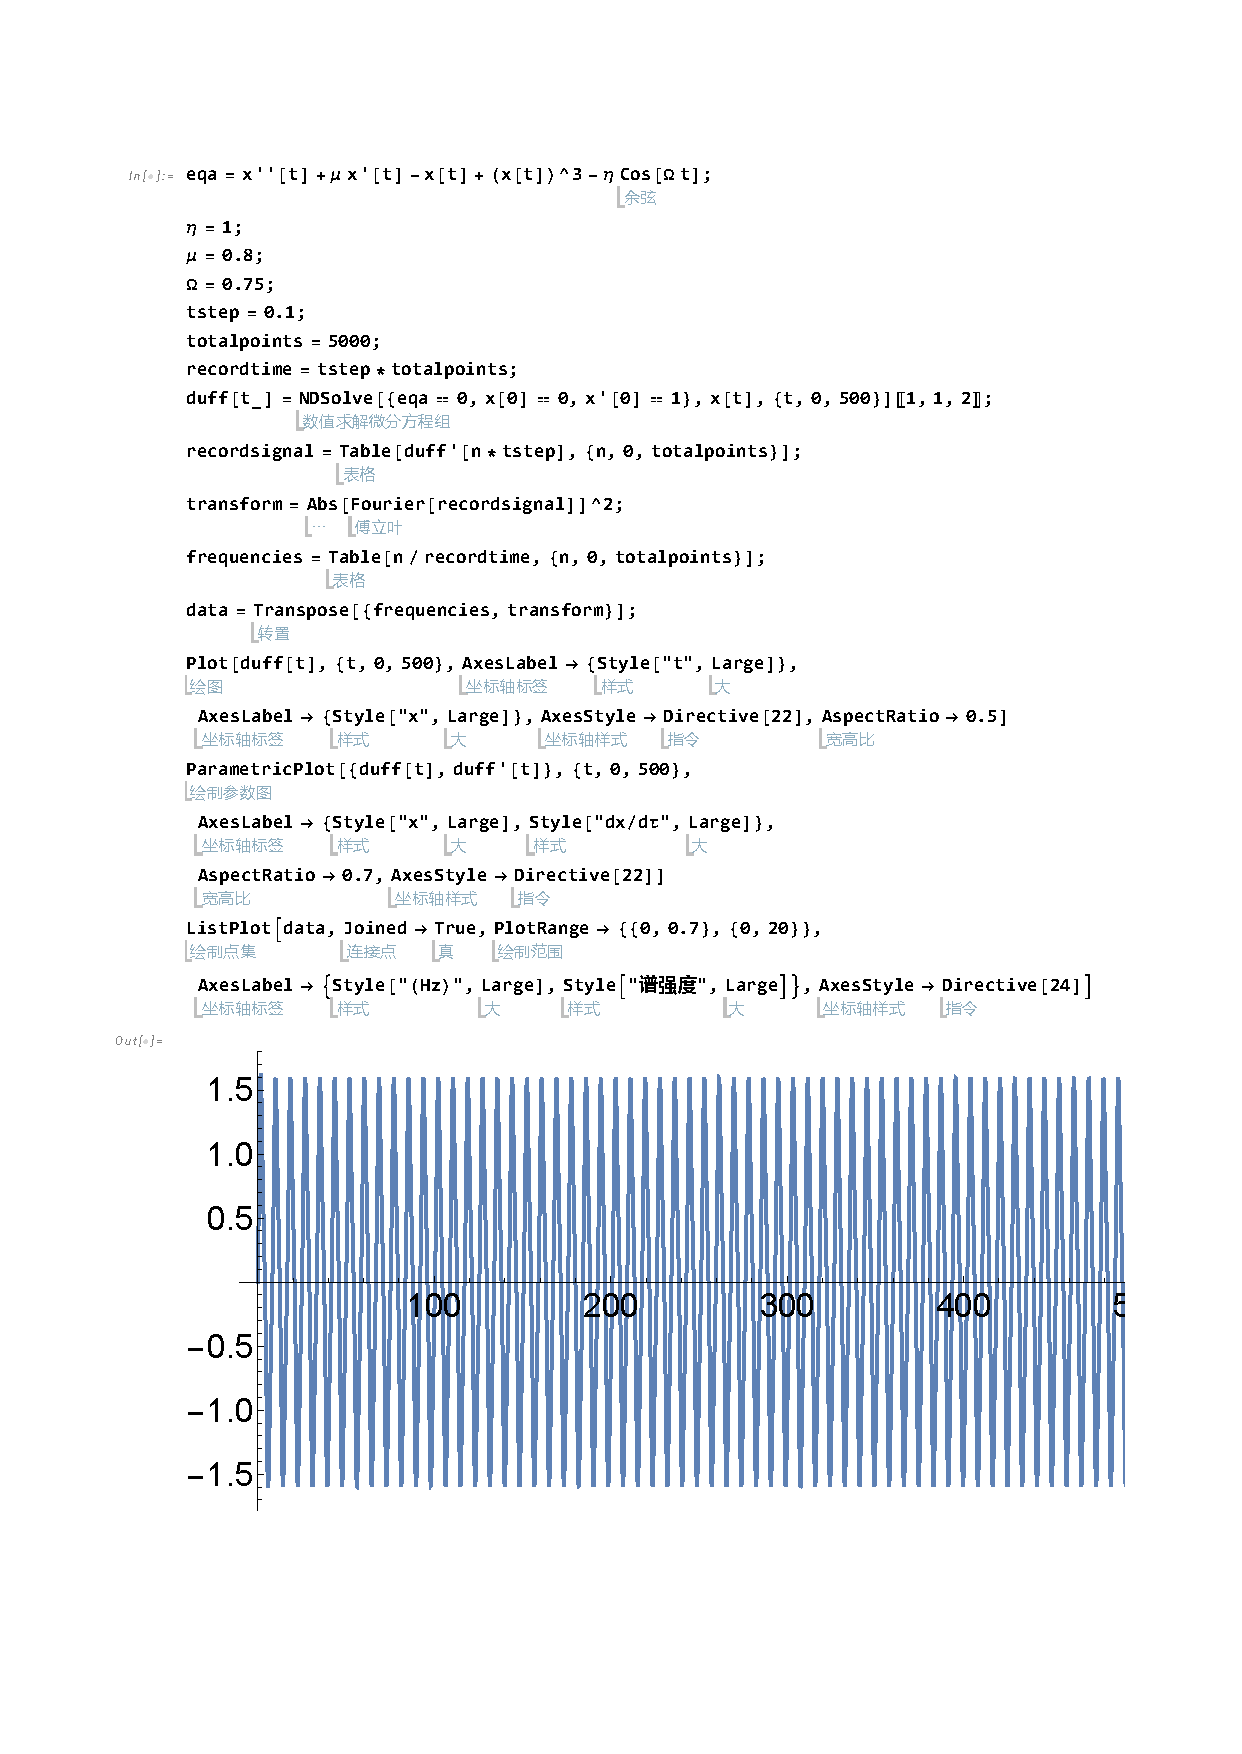
\includepdf[pages=-]{chaos.pdf}
%\subsection*{原件}
%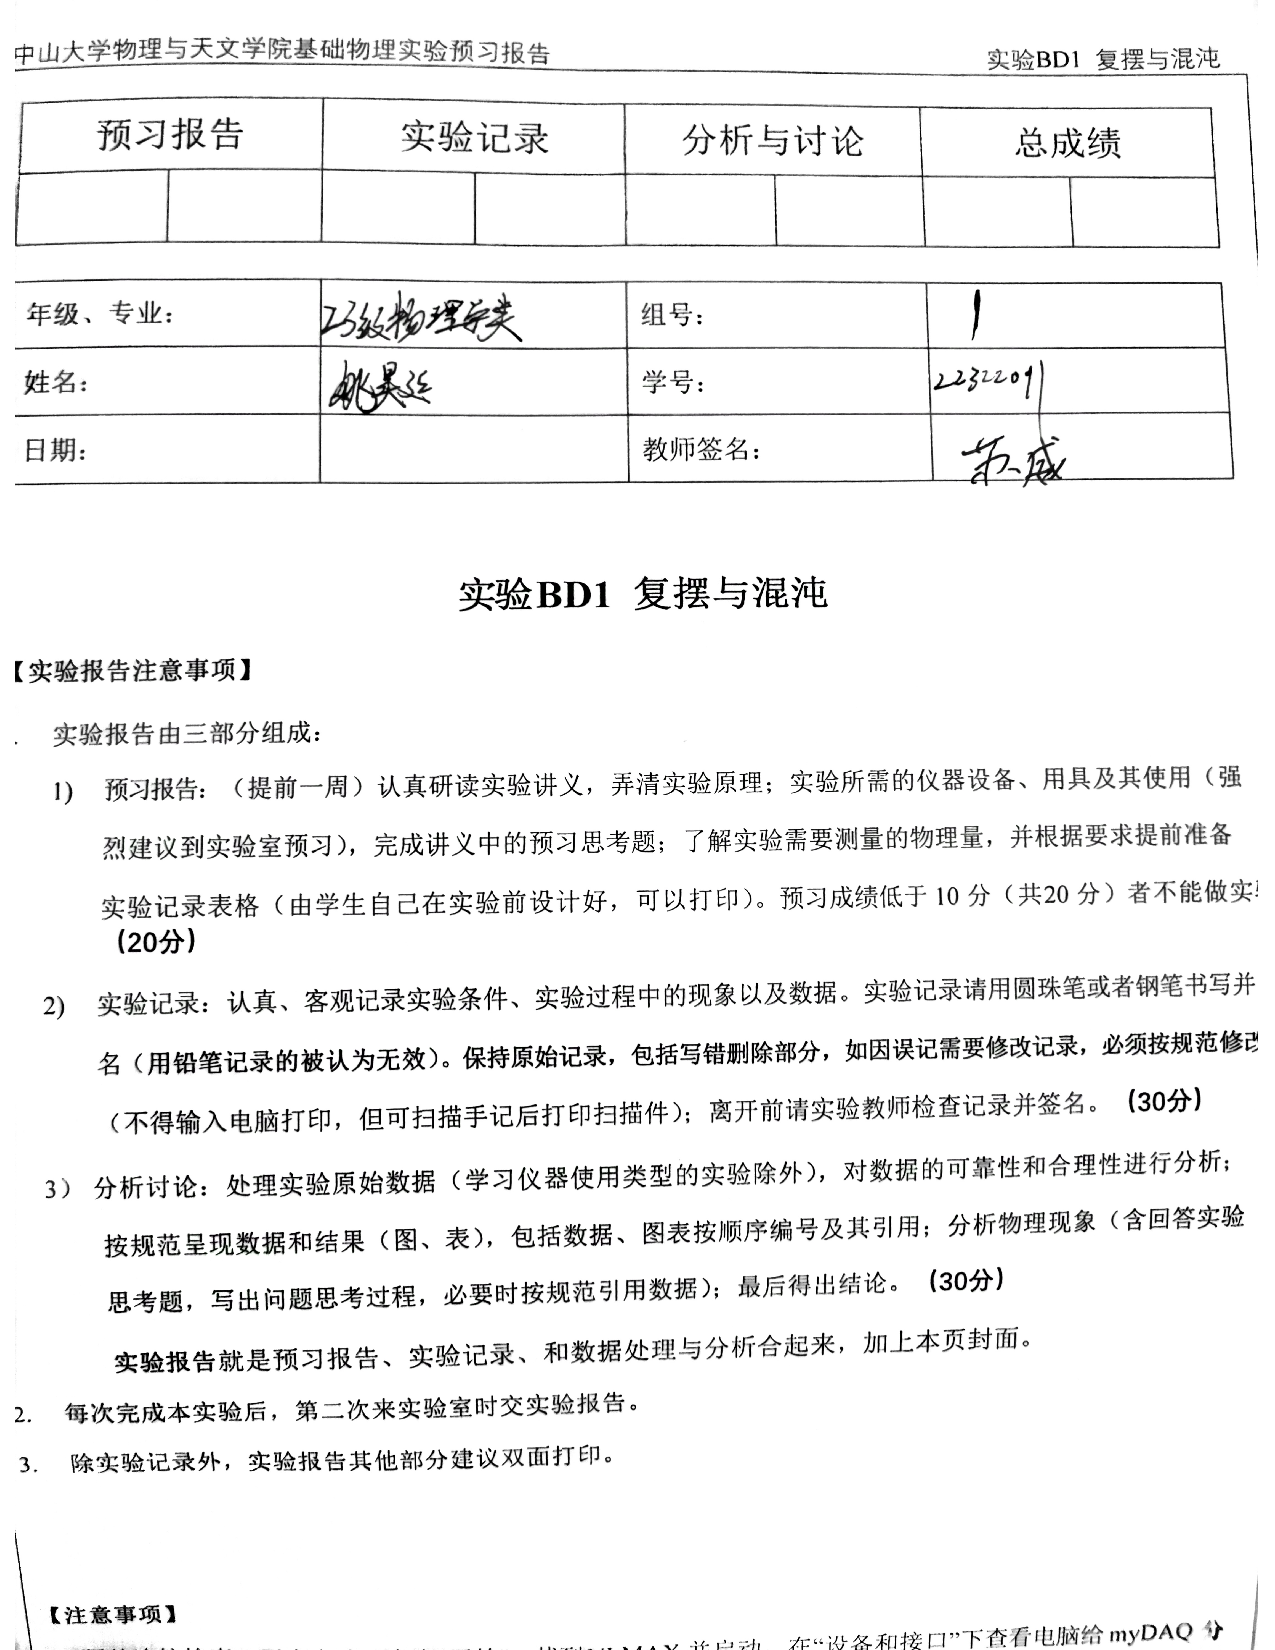
\includepdf[pages=-]{实验3原件.pdf}
%\begin{figure}[H]
%	\centering
%	\includegraphics[width=\textwidth]{焦距数据.jpg}
	
%\end{figure}
%\begin{figure}[H]
%	\centering
%	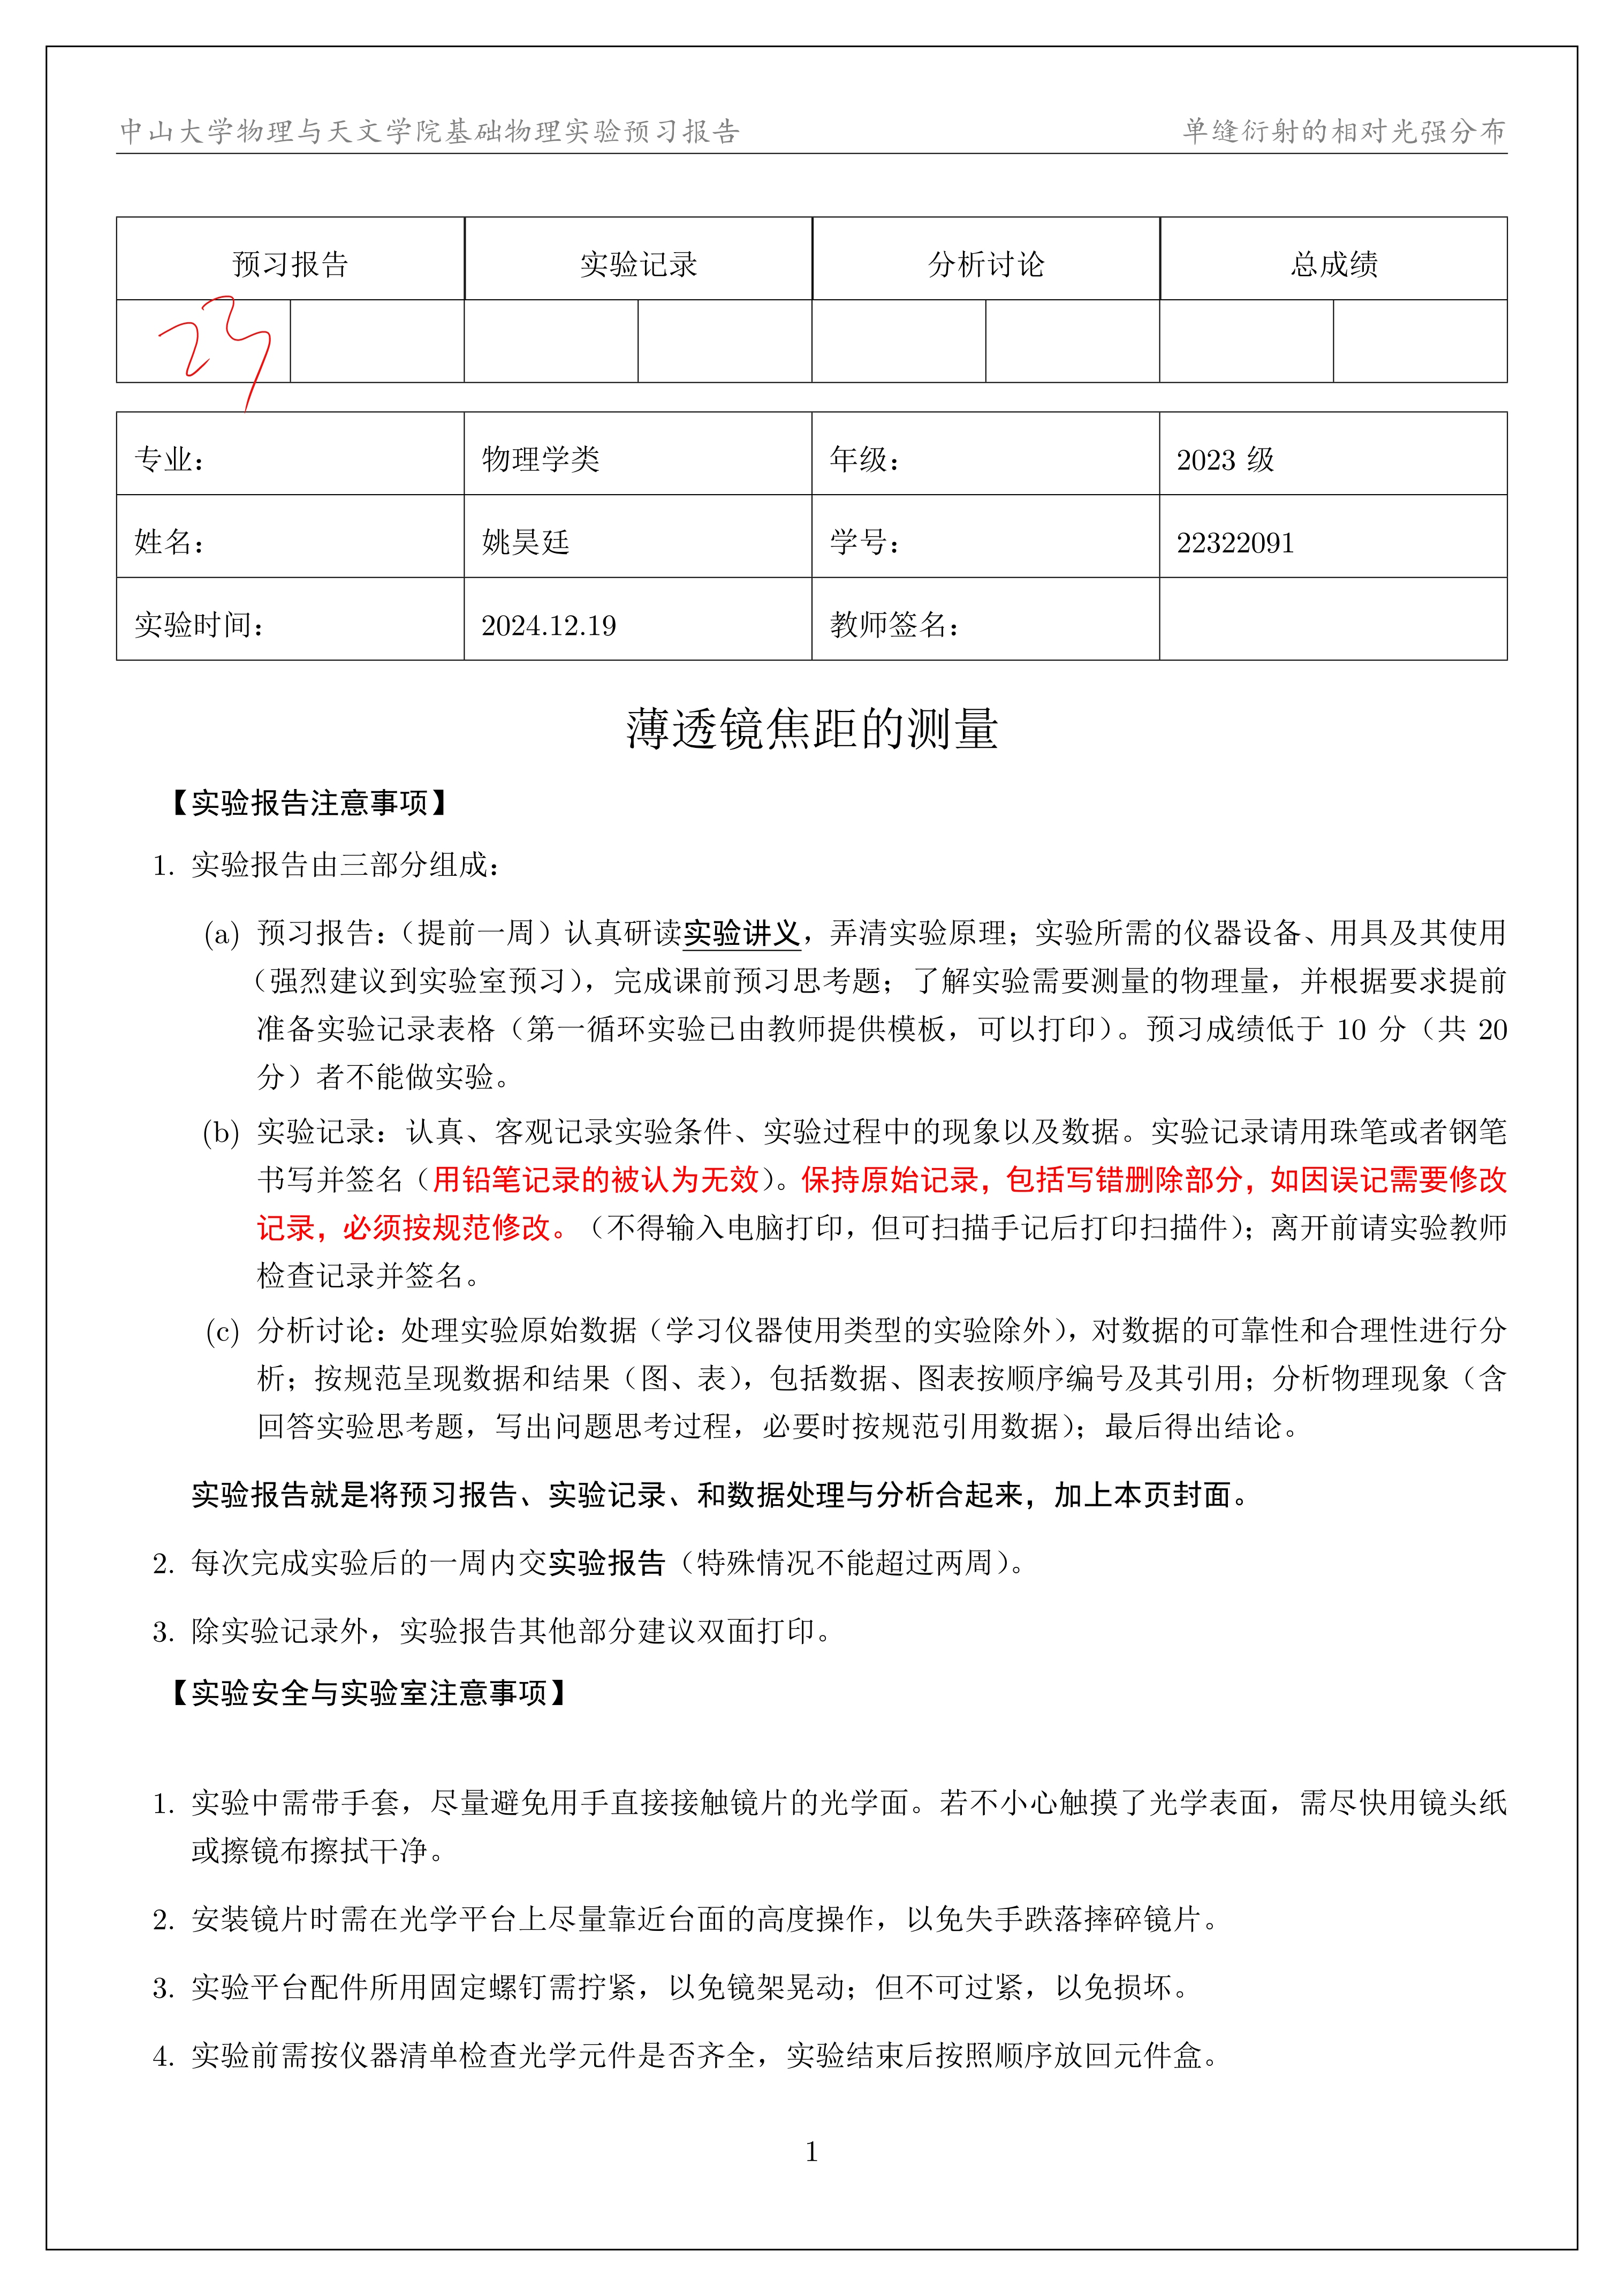
\includegraphics[width=\textwidth]{透镜焦距.jpg}
	
%\end{figure}

%\begin{figure}[H]
%	\centering
%	\includegraphics[width=0.4\textwidth]{单缝原件1.jpg}
%	\includegraphics[width=0.4\textwidth]{单缝原件2.jpg}
%	\includegraphics[width=0.4\textwidth]{单缝原件3.jpg}
%	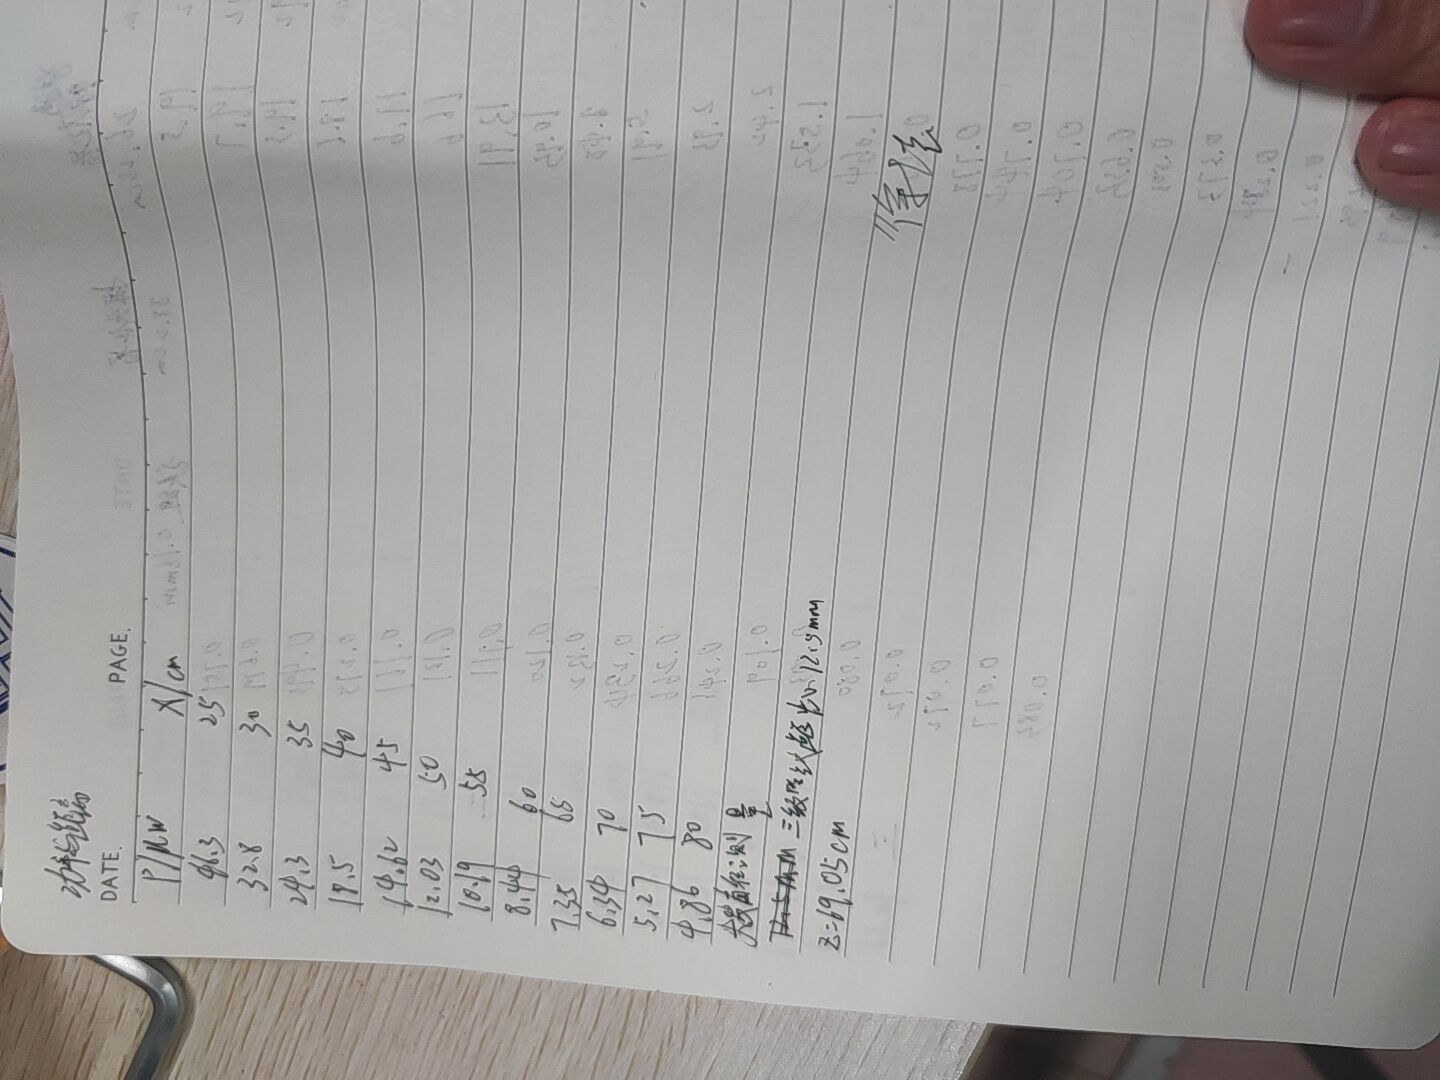
\includegraphics[width=0.4\textwidth]{单缝原件4.jpg}
%\end{figure}
%\subsection*{桌面}
%\begin{figure}[H]
%	\includegraphics[width=0.95\textwidth]{焦距桌面.jpg}
%\end{figure}
\end{document}
%